% !TEX root = ../main.tex

%---------------------------------------------------------------------
%   正文
%---------------------------------------------------------------------
\setcounter{page}{1}
\pagenumbering{arabic}


% section标题左对齐
\titleformat{\section}{\raggedright\Large\bfseries}{\thesection}{1em}{}

\section{Experimental Purpose}

It's the experimental purpose. It's the experimental purpose. It's the experimental purpose. It's the experimental purpose. It's the experimental purpose.
It's the experimental purpose. It's the experimental purpose. It's the experimental purpose. It's the experimental purpose. It's the experimental purpose.


\begin{figure}[!htp]
    \centering
    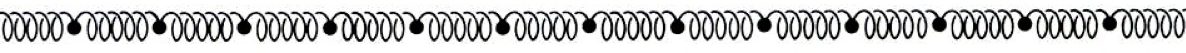
\includegraphics[width=10cm]{Figures/atomic_chain.png}
    \caption{Schematic diagram of 1D periodic atomic chain}
    \label{fig:atomic-chain}
\end{figure}

\section{Experimental Method}\label{sec:exp-method}

It's the experimental method. It's the experimental method. It's the experimental method. It's the experimental method. It's the experimental method.
It's the experimental method. It's the experimental method. It's the experimental method. It's the experimental method. It's the experimental method.


Unnumbered equation:
\begin{equation*}
    E_p = \frac{1}{2} k x^2
\end{equation*}

Numbered equation, such as equation ~\ref{eq:kinetic-energy}。
\begin{equation}
    E_k = \frac{1}{2} m v^2
    \label{eq:kinetic-energy}
\end{equation}


一些数学直立体:
\begin{itemize}
  \item 微分符号 $\dd$:\cs{dd}
  \item 圆周率 $\uppi$:\cs{uppi}
  \item 自然对数的底 $\ee$:\cs{ee}
  \item 虚数单位 $\ii$, $\jj$:\cs{ii} \cs{jj}
\end{itemize}


\section{Experimental Content}

\subsection{Content 1}

实验方法见第~\ref{sec:exp-method}~节。

It's the experimental content 1. It's the experimental content 1. It's the experimental content 1. It's the experimental content 1. 
It's the experimental content 1. It's the experimental content 1. It's the experimental content 1. It's the experimental content 1. 


三线表,如表~\ref{tab:exp-data}。

\begin{longtable}[c]{ccc}
    % \label 后面需要加 \\,否则会报错
    \caption{实验数据}
    \label{tab:exp-data} \\
    \toprule
    \textbf{编号} & \textbf{物理量} & \textbf{数值} \\
    \midrule
    \endhead
    1 & $m$ & 0.1 \\
    2 & $k$ & 1.0 \\
    3 & $x$ & 0.2 \\
    \bottomrule
\end{longtable}



\subsection{Content 2}

具体代码见附录~\ref{sec:appendix-1}。

It's the experimental content 2. It's the experimental content 2. It's the experimental content 2. It's the experimental content 2. 
It's the experimental content 2. It's the experimental content 2. It's the experimental content 2. It's the experimental content 2. 

单张图,如图~\ref{fig:single-figure}。
\begin{figure}[!htp]
    \centering
    
\includegraphics[width=4cm]{Icons/badge_sjtu.png}
    \caption{单张图}
    \label{fig:single-figure}
\end{figure}


两张图并排且共用图题,如图~\ref{fig:two-figures}。
\begin{figure}[!htp]
    \centering
    
\includegraphics[height=2cm]{Icons/badge_sjtu.png}
    \hspace{1cm}
    
\includegraphics[height=2cm]{Icons/badge_sjtu.png}
    \caption{两张图并排}
    \label{fig:two-figures}
\end{figure}


\section{分析与讨论}

这里是分析与讨论。这里是分析与讨论。这里是分析与讨论。这里是分析与讨论。这里是分析与讨论。
这里是分析与讨论。这里是分析与讨论。这里是分析与讨论。这里是分析与讨论。这里是分析与讨论。


文献引用测试:学位论文\cite{Zhang1998},专利文献\cite{Jiang1989,HBLZ2001},
专著中析出的文献\cite{Cheng1999,GBT2659},期刊中析出的文献\cite{Li1999,Li2000},
报纸中析出的文献\cite{Ding2000}, 电子文献\cite{Jiang1999,Christine1998,Xiao2001}。
多个文献引用\cite{Zhang1998,Jiang1999,Christine1998,Xiao2001}。


\section{结论}

这里是结论。这里是结论。这里是结论。这里是结论。这里是结论。
这里是结论。这里是结论。这里是结论。这里是结论。这里是结论。


\begin{itemize}
    \item 这里是结论1。
    \item 这里是结论2。
    \item 这里是结论3。
\end{itemize}


\newpage
